\documentclass{article}

% content/resources/templates/preamble.tex
\usepackage[margin=0.6in]{geometry}
\author{Milav Dabgar}
\usepackage{amsmath,amssymb,amsthm}
\usepackage{booktabs}
\usepackage{multirow}
\usepackage{xcolor}
\usepackage{tcolorbox}
\tcbuselibrary{breakable,skins}
\usepackage[colorlinks=true,linkcolor=blue]{hyperref}
\usepackage{titlesec}
\usepackage{enumitem}
\usepackage{tikz}
\usepackage{pgfplots}
\usepackage{circuitikz}
\usepackage[version=4]{mhchem}
\usepackage{longtable}
\usepackage{array}
\usepackage{float}
\usepackage{caption}
\usepackage{listings}

\lstset{
  basicstyle=\small\ttfamily,
  breaklines=true,
  breakatwhitespace=false,
  postbreak=\mbox{\textcolor{red}{$\hookrightarrow$}\space},
  float=false,
  numbers=left,
  numberstyle=\tiny\color{gray},
  numbersep=10pt,
  xleftmargin=2em,
  keywordstyle=\color{blue},
  commentstyle=\color{green!60!black},
  stringstyle=\color{purple},
  backgroundcolor=\color{gray!5},
  showstringspaces=false,
  tabsize=2,
  captionpos=b,
  keepspaces=true,
  columns=flexible
}

\pgfplotsset{compat=1.18}
\usetikzlibrary{shapes,arrows,positioning,calc,patterns,decorations.pathmorphing,decorations.markings,arrows.meta}

% Color scheme
\definecolor{headcolor}{RGB}{0,102,204}
\definecolor{keycolor}{RGB}{220,20,60}
\definecolor{solutioncolor}{RGB}{34,139,34}
\definecolor{mnemoniccolor}{RGB}{148,0,211}
\definecolor{codecolor}{RGB}{0,0,100}

% Spacing
\setlength{\parskip}{3pt}
\setlist[itemize]{nosep}
\setlist[enumerate]{nosep}

% Title formatting
\titleformat{\section}{\Large\bfseries\color{headcolor}}{\thesection}{1em}{}
\titleformat{\subsection}{\large\bfseries\color{headcolor}}{\thesubsection}{1em}{}

% Pandoc tightlist compatibility
\providecommand{\tightlist}{%
  \setlength{\itemsep}{0pt}\setlength{\parskip}{0pt}}

% Pandoc longtable compatibility
\newcounter{none}
\def\thenone{}


% content/resources/templates/english-boxes.tex

% Custom environments
\newtcolorbox{solutionbox}{
 breakable,
 enhanced,
 colback=solutioncolor!5!white,
 colframe=solutioncolor!75!black,
 fonttitle=\bfseries,
 title=Solution
}

\newtcolorbox{solutionboxnobreak}{
 colback=solutioncolor!5!white,
 colframe=solutioncolor!75!black,
 fonttitle=\bfseries,
 title=Solution
}

\newtcolorbox{keyformula}{
 breakable,
 enhanced,
 colback=keycolor!5!white,
 colframe=keycolor!75!black,
 fonttitle=\bfseries,
 title=Key Formula
}

\newtcolorbox{mnemonicboxenv}{
 breakable,
 enhanced,
 colback=mnemoniccolor!5!white,
 colframe=mnemoniccolor!75!black,
 fonttitle=\bfseries,
 title=Mnemonic
}

\newcommand{\mnemonicbox}[1]{%
  \begin{mnemonicboxenv}
    #1
  \end{mnemonicboxenv}
}


% Custom commands for GTU solutions
% This file defines semantic commands for consistent formatting

% Question command with automatic formatting
\newcommand{\question}[2]{%
  \section*{Question #1}%
  \textbf{#2}%
}

% OR question variant
\newcommand{\questionor}[2]{%
  \section*{Question #1 OR}%
  \textbf{#2}%
}

% Proper table environment with caption
\newenvironment{answertable}[1]{%
  \begin{table}[htbp]
  \centering
  \caption{#1}
}{%
  \end{table}
}

% Proper figure environment for diagrams
\newenvironment{answerdiagram}[1]{%
  \begin{figure}[htbp]
  \centering
  \caption{#1}
}{%
  \end{figure}
}

% Semantic markup for key terms
\newcommand{\keyword}[1]{\textbf{#1}}
\newcommand{\code}[1]{\texttt{#1}}
\newcommand{\classname}[1]{\texttt{#1}}
\newcommand{\methodname}[1]{\texttt{#1}}

% Proper quotation marks
\newcommand{\mnemonic}[1]{``#1''}


\title{Cyber Security and Digital Forensics (4361601) - Summer 2025 Solution}
\date{May 8, 2025}

\begin{document}
\maketitle

\questionmarks{1(a)}{3}{Give comparison between Public key and Private Key cryptography.}
\begin{solutionbox}
    \begin{answertable}{Key Cryptography Comparison}
    \begin{tabulary}{\textwidth}{|L|L|L|}
        \hline
        \textbf{Aspect} & \textbf{Private Key Cryptography} & \textbf{Public Key Cryptography} \\
        \hline
        \textbf{Key Management} & Same key for encryption/decryption & Different keys for encryption/decryption \\
        \hline
        \textbf{Key Distribution} & Secure channel required & No secure channel needed \\
        \hline
        \textbf{Speed} & Fast processing & Slower than private key \\
        \hline
        \textbf{Security Level} & High if key is secret & High mathematical security \\
        \hline
        \textbf{Example} & DES, AES & RSA, ECC \\
        \hline
    \end{tabulary}
    \end{answertable}

    \begin{mnemonicbox}
    "Private Personal, Public Pair"
    \end{mnemonicbox}
\end{solutionbox}

\questionmarks{1(b)}{4}{Explain CIA Triad in detail.}
\begin{solutionbox}
    CIA Triad is the foundation of information security with three core principles:

    \begin{center}
    \begin{tikzpicture}[node distance=2cm, auto]
        \node [gtu block] (cia) {CIA Triad};
        \node [gtu block, below left of=cia, yshift=-1.5cm, xshift=-1cm] (conf) {Confidentiality};
        \node [gtu block, below of=cia, yshift=-1.5cm] (integ) {Integrity};
        \node [gtu block, below right of=cia, yshift=-1.5cm, xshift=1cm] (avail) {Availability};
        
        \node [gtu block, below of=conf] (privacy) {Data Privacy};
        \node [gtu block, below of=integ] (accuracy) {Data Accuracy};
        \node [gtu block, below of=avail] (access) {System Access};

        \draw [gtu arrow] (cia) -- (conf);
        \draw [gtu arrow] (cia) -- (integ);
        \draw [gtu arrow] (cia) -- (avail);
        \draw [gtu arrow] (conf) -- (privacy);
        \draw [gtu arrow] (integ) -- (accuracy);
        \draw [gtu arrow] (avail) -- (access);
    \end{tikzpicture}
    \end{center}

    \begin{itemize}
        \item \keyword{Confidentiality}: Ensures data is accessible only to authorized users
        \item \keyword{Integrity}: Maintains accuracy and completeness of data
        \item \keyword{Availability}: Ensures systems are accessible when needed
    \end{itemize}

    \begin{mnemonicbox}
    "Can I Access" (Confidentiality, Integrity, Availability)
    \end{mnemonicbox}
\end{solutionbox}

\questionmarks{1(c)}{7}{Explain Md5 algorithm steps.}
\begin{solutionbox}
    MD5 (Message Digest 5) is a cryptographic hash function producing 128-bit hash value.

    \begin{answertable}{MD5 Algorithm Steps}
    \begin{tabulary}{\textwidth}{|L|L|L|}
        \hline
        \textbf{Step} & \textbf{Process} & \textbf{Description} \\
        \hline
        1 & \textbf{Padding} & Add bits to make message length $\equiv$ 448 (mod 512) \\
        \hline
        2 & \textbf{Length Addition} & Append 64-bit length of original message \\
        \hline
        3 & \textbf{Initialize Buffers} & Set four 32-bit buffers (A, B, C, D) \\
        \hline
        4 & \textbf{Process Blocks} & Process message in 512-bit blocks \\
        \hline
        5 & \textbf{Round Functions} & Apply 4 rounds of 16 operations each \\
        \hline
    \end{tabulary}
    \end{answertable}

    \begin{codebox}
\begin{lstlisting}[language=python]
# MD5 Processing Steps
def md5_process():
    # Step 1: Padding
    padded_message = original + padding_bits
    # Step 2: Process in 512-bit chunks  
    for chunk in chunks:
        # Step 3: Apply round functions
        result = round_functions(chunk)
    return final_hash
\end{lstlisting}
    \end{codebox}

    \begin{itemize}
        \item \textbf{Round 1}: F(X,Y,Z) = (X$\land$Y) $\lor$ ($\lnot$X$\land$Z)
        \item \textbf{Round 2}: G(X,Y,Z) = (X$\land$Z) $\lor$ (Y$\land\lnot$Z)
        \item \textbf{Round 3}: H(X,Y,Z) = X$\oplus$Y$\oplus$Z
        \item \textbf{Round 4}: I(X,Y,Z) = Y$\oplus$(X$\lor\lnot$Z)
    \end{itemize}

    \begin{mnemonicbox}
    "My Data Needs Proper Processing" (Message, Digest, Needs, Proper, Processing)
    \end{mnemonicbox}
\end{solutionbox}

\orquestionmarks{1(c)}{7}{List inventors of RSA. Write steps of RSA algorithm.}
\begin{solutionbox}
    \textbf{RSA Inventors:}

    \begin{itemize}
        \item \textbf{Ron Rivest} (MIT)
        \item \textbf{Adi Shamir} (MIT) 
        \item \textbf{Leonard Adleman} (MIT)
    \end{itemize}

    \begin{answertable}{RSA Algorithm Steps}
    \begin{tabulary}{\textwidth}{|L|L|L|}
        \hline
        \textbf{Step} & \textbf{Process} & \textbf{Formula} \\
        \hline
        1 & \textbf{Select Primes} & Choose p, q (large primes) \\
        \hline
        2 & \textbf{Calculate n} & n = p $\times$ q \\
        \hline
        3 & \textbf{Calculate $\phi$(n)} & $\phi$(n) = (p-1) $\times$ (q-1) \\
        \hline
        4 & \textbf{Choose e} & gcd(e, $\phi$(n)) = 1 \\
        \hline
        5 & \textbf{Calculate d} & d $\times$ e $\equiv$ 1 (mod $\phi$(n)) \\
        \hline
        6 & \textbf{Encryption} & C = M$^e$ mod n \\
        \hline
        7 & \textbf{Decryption} & M = C$^d$ mod n \\
        \hline
    \end{tabulary}
    \end{answertable}

    \textbf{Key Pairs:}

    \begin{itemize}
        \item \textbf{Public Key}: (n, e)
        \item \textbf{Private Key}: (n, d)
    \end{itemize}

    \begin{mnemonicbox}
    "RSA: Rivest Shamir Adleman"
    \end{mnemonicbox}
\end{solutionbox}

\questionmarks{2(a)}{3}{Define: Firewall. List limitations of firewall.}
\begin{solutionbox}
    \textbf{Definition:} Firewall is a network security device that monitors and controls incoming/outgoing network traffic based on predetermined security rules.

    \begin{answertable}{Limitations of Firewall}
    \begin{tabulary}{\textwidth}{|L|L|}
        \hline
        \textbf{Limitation} & \textbf{Description} \\
        \hline
        \textbf{Internal Threats} & Cannot protect against insider attacks \\
        \hline
        \textbf{Application Layer} & Limited protection against application-specific attacks \\
        \hline
        \textbf{Performance} & Can slow down network traffic \\
        \hline
        \textbf{Configuration} & Requires proper setup and maintenance \\
        \hline
        \textbf{Encrypted Traffic} & Cannot inspect encrypted content effectively \\
        \hline
    \end{tabulary}
    \end{answertable}

    \begin{mnemonicbox}
    "Fire Walls Limit Internal Protection"
    \end{mnemonicbox}
\end{solutionbox}

\questionmarks{2(b)}{4}{Sketch IPsec Tunnel Mode and Transport mode.}
\begin{solutionbox}
    \textbf{IPsec Modes Comparison:}

    \begin{center}
    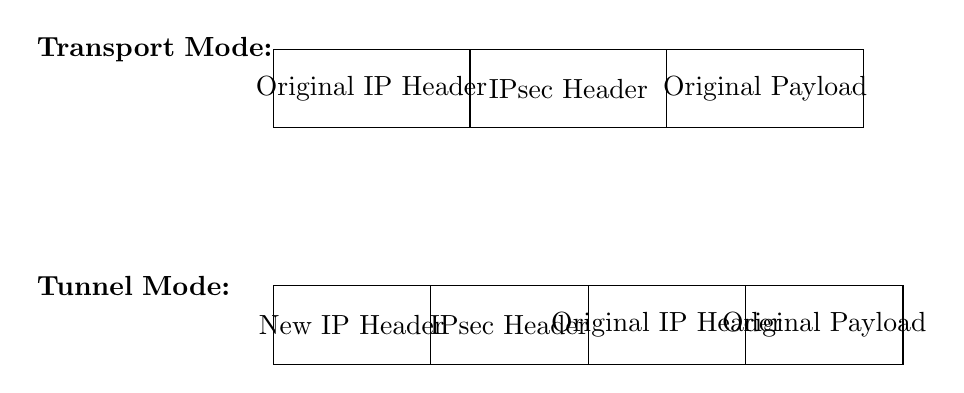
\begin{tikzpicture}[node distance=1cm, auto]
        % Transport Mode
        \node[text width=4cm, align=left] at (-1, 2) {\textbf{Transport Mode:}};
        \draw (0,1) rectangle (2.5,2); \node at (1.25,1.5) {Original IP Header};
        \draw (2.5,1) rectangle (5,2); \node at (3.75,1.5) {IPsec Header};
        \draw (5,1) rectangle (7.5,2); \node at (6.25,1.5) {Original Payload};

        % Tunnel Mode
        \node[text width=4cm, align=left] at (-1, -1) {\textbf{Tunnel Mode:}};
        \draw (0,-2) rectangle (2,-1); \node at (1,-1.5) {New IP Header};
        \draw (2,-2) rectangle (4,-1); \node at (3,-1.5) {IPsec Header};
        \draw (4,-2) rectangle (6,-1); \node at (5,-1.5) {Original IP Header};
        \draw (6,-2) rectangle (8,-1); \node at (7,-1.5) {Original Payload};
    \end{tikzpicture}
    \end{center}

    \begin{answertable}{Key Differences}
    \begin{tabulary}{\textwidth}{|L|L|L|}
        \hline
        \textbf{Aspect} & \textbf{Transport Mode} & \textbf{Tunnel Mode} \\
        \hline
        \textbf{Protection} & Payload only & Entire packet \\
        \hline
        \textbf{Use Case} & End-to-end & Gateway-to-gateway \\
        \hline
        \textbf{Overhead} & Lower & Higher \\
        \hline
        \textbf{IP Header} & Original preserved & New header added \\
        \hline
    \end{tabulary}
    \end{answertable}

    \begin{mnemonicbox}
    "Transport Travels, Tunnel Total"
    \end{mnemonicbox}
\end{solutionbox}

\questionmarks{2(c)}{7}{Explain various types of Active \& Passive attacks in detail.}
\begin{solutionbox}
    \textbf{Attack Classification:}

    \begin{center}
    \begin{tikzpicture}[node distance=2cm, auto]
        \node [gtu block] (root) {Network Attacks};
        \node [gtu block, below left of=root, xshift=-2cm] (active) {Active Attacks};
        \node [gtu block, below right of=root, xshift=2cm] (passive) {Passive Attacks};

        % Active Children
        \node [gtu block, below of=active, xshift=-1.5cm] (mod) {Modification};
        \node [gtu block, below of=active] (fab) {Fabrication};
        \node [gtu block, below of=active, xshift=1.5cm] (int) {Interruption};

        % Passive Children
        \node [gtu block, below of=passive, xshift=-1cm] (eaves) {Eavesdropping};
        \node [gtu block, below of=passive, xshift=1cm] (traffic) {Traffic Analysis};

        \draw [gtu arrow] (root) -- (active);
        \draw [gtu arrow] (root) -- (passive);
        \draw [gtu arrow] (active) -- (mod);
        \draw [gtu arrow] (active) -- (fab);
        \draw [gtu arrow] (active) -- (int);
        \draw [gtu arrow] (passive) -- (eaves);
        \draw [gtu arrow] (passive) -- (traffic);
    \end{tikzpicture}
    \end{center}

    \begin{answertable}{Active Attacks}
    \begin{tabulary}{\textwidth}{|L|L|L|}
        \hline
        \textbf{Type} & \textbf{Description} & \textbf{Example} \\
        \hline
        \textbf{Masquerade} & Impersonating another entity & Fake identity \\
        \hline
        \textbf{Replay} & Retransmitting captured data & Session replay \\
        \hline
        \textbf{Modification} & Altering message content & Data tampering \\
        \hline
        \textbf{DoS} & Denying service availability & Server flooding \\
        \hline
    \end{tabulary}
    \end{answertable}

    \begin{answertable}{Passive Attacks}
    \begin{tabulary}{\textwidth}{|L|L|L|}
        \hline
        \textbf{Type} & \textbf{Description} & \textbf{Impact} \\
        \hline
        \textbf{Eavesdropping} & Listening to communications & Data theft \\
        \hline
        \textbf{Traffic Analysis} & Analyzing communication patterns & Privacy breach \\
        \hline
        \textbf{Monitoring} & Observing network activity & Information gathering \\
        \hline
    \end{tabulary}
    \end{answertable}

    \begin{itemize}
        \item \textbf{Active attacks} modify system resources or data
        \item \textbf{Passive attacks} observe and collect information
        \item \textbf{Detection}: Active attacks easier to detect than passive
    \end{itemize}

    \begin{mnemonicbox}
    "Active Acts, Passive Peeks"
    \end{mnemonicbox}
\end{solutionbox}

\orquestionmarks{2(a)}{3}{Define: Digital Signature. Also discuss various application areas of Digital Signature.}
\begin{solutionbox}
    \textbf{Definition:} Digital Signature is a cryptographic technique that validates authenticity and integrity of digital messages or documents using public key cryptography.

    \begin{answertable}{Application Areas}
    \begin{tabulary}{\textwidth}{|L|L|}
        \hline
        \textbf{Area} & \textbf{Use Case} \\
        \hline
        \textbf{E-commerce} & Online transactions, contracts \\
        \hline
        \textbf{Banking} & Electronic fund transfers, cheques \\
        \hline
        \textbf{Government} & Digital certificates, official documents \\
        \hline
        \textbf{Healthcare} & Patient records, prescriptions \\
        \hline
        \textbf{Legal} & Electronic contracts, court documents \\
        \hline
    \end{tabulary}
    \end{answertable}

    \begin{mnemonicbox}
    "Digital Documents Demand Authentic Approval"
    \end{mnemonicbox}
\end{solutionbox}

\orquestionmarks{2(b)}{4}{Differentiate HTTP \& HTTPS.}
\begin{solutionbox}
    \begin{answertable}{HTTP vs HTTPS}
    \begin{tabulary}{\textwidth}{|L|L|L|}
        \hline
        \textbf{Parameter} & \textbf{HTTP} & \textbf{HTTPS} \\
        \hline
        \textbf{Security} & No encryption & SSL/TLS encryption \\
        \hline
        \textbf{Port} & 80 & 443 \\
        \hline
        \textbf{Protocol} & Hypertext Transfer Protocol & HTTP + SSL/TLS \\
        \hline
        \textbf{Data Protection} & Plain text & Encrypted \\
        \hline
        \textbf{Authentication} & No server verification & Server certificate validation \\
        \hline
        \textbf{Speed} & Faster & Slightly slower \\
        \hline
        \textbf{URL Prefix} & http:// & https:// \\
        \hline
    \end{tabulary}
    \end{answertable}

    \textbf{Diagram:}

    \begin{center}
    \begin{tikzpicture}[node distance=3cm, auto]
        % Client and Server Nodes
        \node [gtu block] (client) {Client};
        \node [gtu block, right of=client, xshift=4cm] (server) {Server};

        % HTTP Path
        \draw [gtu arrow, bend left=20] (client) to node[above] {HTTP: Plain Text} (server);

        % HTTPS Path
        \draw [gtu arrow, bend right=20] (client) to node[below] {HTTPS: Encrypted} (server);
        \node [draw, dashed, fit=(client) (server), label=below:SSL/TLS Layer] {};
    \end{tikzpicture}
    \end{center}

    \begin{mnemonicbox}
    "HTTPS Has Security"
    \end{mnemonicbox}
\end{solutionbox}

\orquestionmarks{2(c)}{7}{Define: Malicious software. Explain Virus, Worm, Keylogger, Trojans in detail.}
\begin{solutionbox}
    \textbf{Definition:} Malicious software (Malware) is any software designed to harm, exploit, or gain unauthorized access to computer systems.

    \begin{answertable}{Types of Malware}
    \begin{tabulary}{\textwidth}{|L|L|L|}
        \hline
        \textbf{Type} & \textbf{Characteristics} & \textbf{Behavior} \\
        \hline
        \textbf{Virus} & Requires host file & Attaches to programs, spreads when executed \\
        \hline
        \textbf{Worm} & Self-replicating & Spreads independently through networks \\
        \hline
        \textbf{Keylogger} & Records keystrokes & Steals passwords and sensitive data \\
        \hline
        \textbf{Trojan} & Disguised as legitimate & Provides backdoor access to attackers \\
        \hline
    \end{tabulary}
    \end{answertable}

    \textbf{Detailed Explanation:}

    \textbf{Virus:}
    \begin{itemize}
        \item Requires host program to execute
        \item Spreads through infected files
        \item Can corrupt or delete data
    \end{itemize}

    \textbf{Worm:}
    \begin{itemize}
        \item Self-propagating malware
        \item Exploits network vulnerabilities
        \item Consumes network bandwidth
    \end{itemize}

    \textbf{Keylogger:}
    \begin{itemize}
        \item Records user keystrokes
        \item Captures login credentials
        \item Can be hardware or software-based
    \end{itemize}

    \textbf{Trojan:}
    \begin{itemize}
        \item Appears as legitimate software
        \item Creates backdoor for remote access
        \item Does not self-replicate
    \end{itemize}

    \begin{mnemonicbox}
    "Viruses Visit, Worms Wander, Keys Captured, Trojans Trick"
    \end{mnemonicbox}
\end{solutionbox}

\questionmarks{3(a)}{3}{Define: Cybercrime. Also discuss needs of Cyber Law.}
\begin{solutionbox}
    \textbf{Definition:} Cybercrime refers to criminal activities carried out using computers, networks, or digital devices as tools or targets.

    \begin{answertable}{Needs of Cyber Law}
    \begin{tabulary}{\textwidth}{|L|L|}
        \hline
        \textbf{Need} & \textbf{Justification} \\
        \hline
        \textbf{Legal Framework} & Establish clear definitions of cyber offenses \\
        \hline
        \textbf{Jurisdiction} & Define authority across geographical boundaries \\
        \hline
        \textbf{Evidence} & Guidelines for digital evidence collection \\
        \hline
        \textbf{Punishment} & Deterrent measures for cybercriminals \\
        \hline
        \textbf{Protection} & Safeguard individual and organizational rights \\
        \hline
    \end{tabulary}
    \end{answertable}

    \begin{mnemonicbox}
    "Cyber Laws Create Legal Protection"
    \end{mnemonicbox}
\end{solutionbox}

\questionmarks{3(b)}{4}{Explain Cyber spying and Cyber theft.}
\begin{solutionbox}
    \textbf{Cyber Spying:}
    \begin{itemize}
        \item \textbf{Definition}: Unauthorized surveillance of digital communications and activities
        \item \textbf{Methods}: Malware, phishing, social engineering
        \item \textbf{Targets}: Government, corporate secrets, personal data
        \item \textbf{Impact}: National security threats, competitive disadvantage
    \end{itemize}

    \textbf{Cyber Theft:}
    \begin{itemize}
        \item \textbf{Definition}: Unauthorized taking of digital assets or information
        \item \textbf{Types}: Identity theft, financial fraud, intellectual property theft
        \item \textbf{Methods}: Hacking, social engineering, insider threats
        \item \textbf{Consequences}: Financial loss, reputation damage
    \end{itemize}

    \begin{answertable}{Comparison Table}
    \begin{tabulary}{\textwidth}{|L|L|L|}
        \hline
        \textbf{Aspect} & \textbf{Cyber Spying} & \textbf{Cyber Theft} \\
        \hline
        \textbf{Purpose} & Information gathering & Asset acquisition \\
        \hline
        \textbf{Detection} & Often undetected & May be noticed \\
        \hline
        \textbf{Duration} & Long-term monitoring & One-time or periodic \\
        \hline
        \textbf{Motivation} & Intelligence/espionage & Financial gain \\
        \hline
    \end{tabulary}
    \end{answertable}

    \begin{mnemonicbox}
    "Spies Spy, Thieves Take"
    \end{mnemonicbox}
\end{solutionbox}

\questionmarks{3(c)}{7}{Explain article section 66 of cyber law.}
\begin{solutionbox}
    \textbf{Section 66 - Computer Related Offences (IT Act 2008):}

    \begin{answertable}{Key Provisions}
    \begin{tabulary}{\textwidth}{|L|L|L|}
        \hline
        \textbf{Sub-section} & \textbf{Offense} & \textbf{Punishment} \\
        \hline
        \textbf{66(1)} & Dishonestly/fraudulently computer resource damage & Up to 3 years imprisonment + fine up to ₹5 lakh \\
        \hline
        \textbf{66A} & Sending offensive messages & Up to 3 years + fine \\
        \hline
        \textbf{66B} & Receiving stolen computer resource & Up to 3 years + fine up to ₹1 lakh \\
        \hline
        \textbf{66C} & Identity theft & Up to 3 years + fine up to ₹1 lakh \\
        \hline
        \textbf{66D} & Cheating by personation using computer & Up to 3 years + fine up to ₹1 lakh \\
        \hline
        \textbf{66E} & Violation of privacy & Up to 3 years + fine up to ₹2 lakh \\
        \hline
        \textbf{66F} & Cyber terrorism & Life imprisonment \\
        \hline
    \end{tabulary}
    \end{answertable}

    \textbf{Detailed Coverage:}

    \textbf{Section 66 Main Offenses:}
    \begin{itemize}
        \item \textbf{Hacking}: Unauthorized access to computer systems
        \item \textbf{Data Theft}: Stealing or copying data without permission
        \item \textbf{System Damage}: Destroying or altering computer data
        \item \textbf{Virus Introduction}: Introducing malicious code
    \end{itemize}

    \textbf{Elements Required:}
    \begin{itemize}
        \item \textbf{Intent}: Dishonest or fraudulent intention
        \item \textbf{Access}: Without permission of owner
        \item \textbf{Damage}: Causing harm to system or data
        \item \textbf{Knowledge}: Awareness of unauthorized access
    \end{itemize}

    \textbf{Legal Framework:}
    \begin{itemize}
        \item \textbf{Cognizable}: Police can arrest without warrant
        \item \textbf{Non-bailable}: Bail at court's discretion
        \item \textbf{Evidence}: Digital evidence admissible in court
    \end{itemize}

    \begin{mnemonicbox}
    "Section 66 Stops Cyber Sins"
    \end{mnemonicbox}
\end{solutionbox}

\orquestionmarks{3(a)}{3}{Explain Cyber terrorism.}
\begin{solutionbox}
    \textbf{Definition:} Cyber terrorism involves the use of digital technologies to create fear, disruption, or harm for political, religious, or ideological purposes.

    \begin{answertable}{Characteristics}
    \begin{tabulary}{\textwidth}{|L|L|}
        \hline
        \textbf{Aspect} & \textbf{Description} \\
        \hline
        \textbf{Target} & Critical infrastructure, government systems \\
        \hline
        \textbf{Method} & DDoS attacks, system infiltration, data destruction \\
        \hline
        \textbf{Motivation} & Political, religious, ideological goals \\
        \hline
        \textbf{Impact} & Public fear, economic disruption, national security \\
        \hline
    \end{tabulary}
    \end{answertable}

    \textbf{Examples:}
    \begin{itemize}
        \item Power grid attacks
        \item Transportation system disruption
        \item Financial system targeting
    \end{itemize}

    \begin{mnemonicbox}
    "Terror Through Technology"
    \end{mnemonicbox}
\end{solutionbox}

\orquestionmarks{3(b)}{4}{Explain Cyber bullying \& Cyber stalking.}
\begin{solutionbox}
    \textbf{Cyber Bullying:}
    \begin{itemize}
        \item \textbf{Definition}: Using digital platforms to harass, intimidate, or harm others
        \item \textbf{Platforms}: Social media, messaging apps, online forums
        \item \textbf{Characteristics}: Repetitive, intentional harm, power imbalance
        \item \textbf{Impact}: Psychological trauma, depression, social isolation
    \end{itemize}

    \textbf{Cyber Stalking:}
    \begin{itemize}
        \item \textbf{Definition}: Persistent online harassment causing fear or emotional distress
        \item \textbf{Methods}: Unwanted messages, tracking, identity theft
        \item \textbf{Duration}: Long-term, continuous behavior
        \item \textbf{Legal}: Criminal offense in many jurisdictions
    \end{itemize}

    \begin{answertable}{Comparison}
    \begin{tabulary}{\textwidth}{|L|L|L|}
        \hline
        \textbf{Aspect} & \textbf{Cyber Bullying} & \textbf{Cyber Stalking} \\
        \hline
        \textbf{Duration} & Episodes & Persistent \\
        \hline
        \textbf{Age Group} & Mainly minors & All ages \\
        \hline
        \textbf{Motivation} & Social dominance & Obsession/control \\
        \hline
        \textbf{Platform} & Public/semi-public & Private/public \\
        \hline
    \end{tabulary}
    \end{answertable}

    \begin{mnemonicbox}
    "Bullies Bother, Stalkers Stalk"
    \end{mnemonicbox}
\end{solutionbox}

\orquestionmarks{3(c)}{7}{Explain article section 67 of cyber law.}
\begin{solutionbox}
    \textbf{Section 67 - Publishing Obscene Information (IT Act 2008):}

    \begin{answertable}{Main Provisions}
    \begin{tabulary}{\textwidth}{|L|L|L|}
        \hline
        \textbf{Section} & \textbf{Content} & \textbf{Punishment} \\
        \hline
        \textbf{67} & Publishing obscene material & First conviction: 3 years + ₹5 lakh fine \\
        \hline
        \textbf{67A} & Sexually explicit material & Up to 5 years + ₹10 lakh fine \\
        \hline
        \textbf{67B} & Child pornography & First: 5 years + ₹10 lakh, Subsequent: 7 years + ₹10 lakh \\
        \hline
        \textbf{67C} & Intermediate liability & Failure to remove illegal content \\
        \hline
    \end{tabulary}
    \end{answertable}

    \textbf{Key Elements:}

    \textbf{Section 67 - Obscenity:}
    \begin{itemize}
        \item \textbf{Publishing}: Making available in electronic form
        \item \textbf{Content}: Lascivious, sexually explicit material
        \item \textbf{Medium}: Website, email, social media
        \item \textbf{Intent}: Corrupt or deprave viewers
    \end{itemize}

    \textbf{Section 67A - Sexually Explicit:}
    \begin{itemize}
        \item \textbf{Enhanced punishment} for explicit sexual content
        \item \textbf{Broader scope} than general obscenity
        \item \textbf{Commercial purpose} considered aggravating factor
    \end{itemize}

    \textbf{Section 67B - Child Protection:}
    \begin{itemize}
        \item \textbf{Zero tolerance} for child exploitation
        \item \textbf{Strict liability} for possession and distribution
        \item \textbf{Higher penalties} reflecting seriousness
        \item \textbf{Age verification} requirements for platforms
    \end{itemize}

    \textbf{Defenses Available:}
    \begin{itemize}
        \item \textbf{Scientific/educational} purpose
        \item \textbf{Artistic merit} consideration
        \item \textbf{Private viewing} in some cases
        \item \textbf{Lack of knowledge} about content nature
    \end{itemize}

    \textbf{Digital Evidence Requirements:}
    \begin{itemize}
        \item \textbf{Chain of custody} maintenance
        \item \textbf{Technical authenticity} proof
        \item \textbf{Source identification} methods
        \item \textbf{Preservation} of electronic evidence
    \end{itemize}

    \begin{mnemonicbox}
    "Section 67 Stops Shameful Sharing"
    \end{mnemonicbox}
\end{solutionbox}

\questionmarks{4(a)}{3}{Discuss types of Hackers.}
\begin{solutionbox}
    \textbf{Hacker Classification:}

    \begin{answertable}{Hacker Types}
    \begin{tabulary}{\textwidth}{|L|L|L|}
        \hline
        \textbf{Type} & \textbf{Motivation} & \textbf{Activities} \\
        \hline
        \textbf{White Hat} & Ethical security testing & Authorized penetration testing \\
        \hline
        \textbf{Black Hat} & Malicious intent & Illegal system breaking \\
        \hline
        \textbf{Gray Hat} & Mixed motivations & Unauthorized but non-malicious \\
        \hline
        \textbf{Script Kiddie} & Recognition/fun & Using existing tools \\
        \hline
        \textbf{Hacktivist} & Political/social causes & Protest through hacking \\
        \hline
    \end{tabulary}
    \end{answertable}

    \textbf{Detailed Types:}

    \begin{itemize}
        \item \textbf{White Hat}: Ethical hackers, security professionals
        \item \textbf{Black Hat}: Cybercriminals seeking profit or damage
        \item \textbf{Gray Hat}: Between ethical and malicious
    \end{itemize}

    \begin{mnemonicbox}
    "Hats Have Hacker Hierarchy"
    \end{mnemonicbox}
\end{solutionbox}

\questionmarks{4(b)}{4}{Explain RAT.}
\begin{solutionbox}
    \textbf{RAT (Remote Administration Tool):}

    \textbf{Definition:} Software that allows remote control of a computer system, often used maliciously for unauthorized access.

    \begin{answertable}{Characteristics}
    \begin{tabulary}{\textwidth}{|L|L|}
        \hline
        \textbf{Feature} & \textbf{Description} \\
        \hline
        \textbf{Remote Control} & Complete system access from distance \\
        \hline
        \textbf{Stealth Mode} & Hidden from user detection \\
        \hline
        \textbf{Data Theft} & File access and transfer capabilities \\
        \hline
        \textbf{Keylogging} & Keystroke recording \\
        \hline
        \textbf{Screen Capture} & Desktop monitoring \\
        \hline
    \end{tabulary}
    \end{answertable}

    \textbf{Common RATs:}
    \begin{itemize}
        \item \textbf{BackOrifice}
        \item \textbf{NetBus}
        \item \textbf{DarkComet}
        \item \textbf{Poison Ivy}
    \end{itemize}

    \textbf{Detection Methods:}
    \begin{itemize}
        \item Antivirus software
        \item Network monitoring
        \item Process analysis
        \item Behavioral detection
    \end{itemize}

    \begin{mnemonicbox}
    "RATs Run Remote Access Tactics"
    \end{mnemonicbox}
\end{solutionbox}

\questionmarks{4(c)}{7}{Explain Five Steps of Hacking.}
\begin{solutionbox}
    \textbf{The Five-Phase Hacking Methodology:}

    \begin{center}
    \begin{tikzpicture}[node distance=2.2cm, auto]
        \node [gtu block] (recon) {1. Reconnaissance};
        \node [gtu block, right of=recon] (scan) {2. Scanning};
        \node [gtu block, right of=scan] (gain) {3. Gaining Access};
        \node [gtu block, right of=gain] (maint) {4. Maintaining Access};
        \node [gtu block, right of=maint] (cover) {5. Covering Tracks};

        \draw [gtu arrow] (recon) -- (scan);
        \draw [gtu arrow] (scan) -- (gain);
        \draw [gtu arrow] (gain) -- (maint);
        \draw [gtu arrow] (maint) -- (cover);
    \end{tikzpicture}
    \end{center}

    \begin{answertable}{Detailed Steps}
    \begin{tabulary}{\textwidth}{|L|L|L|L|}
        \hline
        \textbf{Phase} & \textbf{Purpose} & \textbf{Techniques} & \textbf{Tools} \\
        \hline
        \textbf{1. Reconnaissance} & Information Gathering & OSINT, Social Engineering & Google, Shodan, WHOIS \\
        \hline
        \textbf{2. Scanning} & Identify Vulnerabilities & Port scanning, Network mapping & Nmap, Nessus \\
        \hline
        \textbf{3. Gaining Access} & Exploit Vulnerabilities & Password attacks, Code injection & Metasploit, Hydra \\
        \hline
        \textbf{4. Maintaining Access} & Persistent Control & Backdoors, Rootkits & RATs, Trojans \\
        \hline
        \textbf{5. Covering Tracks} & Hide Evidence & Log deletion, Steganography & CCleaner, File wipers \\
        \hline
    \end{tabulary}
    \end{answertable}

    \textbf{Phase 1 - Reconnaissance:}
    \begin{itemize}
        \item \textbf{Passive}: Public information gathering
        \item \textbf{Active}: Direct target interaction
        \item \textbf{Goal}: Map target infrastructure
    \end{itemize}

    \textbf{Phase 2 - Scanning:}
    \begin{itemize}
        \item \textbf{Network scanning}: Live system identification
        \item \textbf{Port scanning}: Service discovery  
        \item \textbf{Vulnerability scanning}: Weakness identification
    \end{itemize}

    \textbf{Phase 3 - Gaining Access:}
    \begin{itemize}
        \item \textbf{Exploitation}: Vulnerability utilization
        \item \textbf{Authentication attacks}: Password cracking
        \item \textbf{Privilege escalation}: Higher access levels
    \end{itemize}

    \textbf{Phase 4 - Maintaining Access:}
    \begin{itemize}
        \item \textbf{Backdoor installation}: Future access
        \item \textbf{System modification}: Persistence mechanisms
        \item \textbf{Data collection}: Information harvesting
    \end{itemize}

    \textbf{Phase 5 - Covering Tracks:}
    \begin{itemize}
        \item \textbf{Log manipulation}: Evidence removal
        \item \textbf{File deletion}: Trace elimination
        \item \textbf{Timeline modification}: Activity concealment
    \end{itemize}

    \begin{mnemonicbox}
    "Real Smart Guys Make Choices" (Reconnaissance, Scanning, Gaining, Maintaining, Covering)
    \end{mnemonicbox}
\end{solutionbox}

\orquestionmarks{4(a)}{3}{Explain Brute force attack.}
\begin{solutionbox}
    \textbf{Definition:} Brute force attack is a trial-and-error method used to decode encrypted data by systematically trying all possible combinations.

    \begin{answertable}{Characteristics}
    \begin{tabulary}{\textwidth}{|L|L|}
        \hline
        \textbf{Aspect} & \textbf{Description} \\
        \hline
        \textbf{Method} & Exhaustive key search \\
        \hline
        \textbf{Time} & Computationally intensive \\
        \hline
        \textbf{Success} & Guaranteed but time-consuming \\
        \hline
        \textbf{Target} & Passwords, encryption keys \\
        \hline
        \textbf{Tools} & Automated software \\
        \hline
    \end{tabulary}
    \end{answertable}

    \textbf{Types:}
    \begin{itemize}
        \item \textbf{Simple Brute Force}: All possible combinations
        \item \textbf{Dictionary Attack}: Common passwords
        \item \textbf{Hybrid Attack}: Dictionary + variations
    \end{itemize}

    \begin{mnemonicbox}
    "Brute Force Breaks By Trying"
    \end{mnemonicbox}
\end{solutionbox}

\orquestionmarks{4(b)}{4}{Define: Vulnerability, Threat, Exploit}
\begin{solutionbox}
    \textbf{Security Terminology:}

    \begin{answertable}{Term Definitions}
    \begin{tabulary}{\textwidth}{|L|L|L|}
        \hline
        \textbf{Term} & \textbf{Definition} & \textbf{Example} \\
        \hline
        \textbf{Vulnerability} & Weakness in system/software & Unpatched software bug \\
        \hline
        \textbf{Threat} & Potential danger to asset & Malicious hacker \\
        \hline
        \textbf{Exploit} & Code taking advantage of vulnerability & Buffer overflow attack \\
        \hline
    \end{tabulary}
    \end{answertable}

    \textbf{Relationship:}

    \begin{center}
    \begin{tikzpicture}[node distance=3cm, auto]
        \node [gtu block] (vuln) {Vulnerability};
        \node [gtu block, right of=vuln] (exploit) {Exploit};
        \node [gtu block, left of=vuln] (threat) {Threat};

        \draw [gtu arrow] (threat) -- node [above] {Uses} (exploit);
        \draw [gtu arrow] (exploit) -- node [above] {Targets} (vuln);
        
        \node [gtu block, below of=threat, yshift=1cm] (hacker) {Hacker};
        \node [gtu block, below of=exploit, yshift=1cm] (code) {Attack Code};
        \node [gtu block, below of=vuln, yshift=1cm] (weak) {System Weakness};

        \draw [gtu arrow, dashed] (threat) -- (hacker);
        \draw [gtu arrow, dashed] (exploit) -- (code);
        \draw [gtu arrow, dashed] (vuln) -- (weak);
    \end{tikzpicture}
    \end{center}

    \textbf{Examples:}
    \begin{itemize}
        \item \textbf{Vulnerability}: SQL injection flaw
        \item \textbf{Threat}: Cybercriminal
        \item \textbf{Exploit}: SQL injection payload
    \end{itemize}

    \textbf{Risk Formula:}
    Risk = Threat $\times$ Vulnerability $\times$ Asset Value

    \begin{mnemonicbox}
    "Threats Target Vulnerable Exploits"
    \end{mnemonicbox}
\end{solutionbox}

\orquestionmarks{4(c)}{7}{Explain any three basic commands of kali Linux with suitable example.}
\begin{solutionbox}
    \textbf{Essential Kali Linux Commands:}

    \textbf{1. NMAP (Network Mapper):}
    \begin{codebox}
\begin{lstlisting}[language=bash]
# Port scanning
nmap -sS target_ip
nmap -A -T4 192.168.1.1
\end{lstlisting}
    \end{codebox}

    \begin{answertable}{Nmap Options}
    \begin{tabulary}{\textwidth}{|L|L|L|}
        \hline
        \textbf{Option} & \textbf{Purpose} & \textbf{Example} \\
        \hline
        \textbf{-sS} & SYN scan & nmap -sS 192.168.1.1 \\
        \hline
        \textbf{-A} & Aggressive scan & nmap -A target.com \\
        \hline
        \textbf{-p} & Specific ports & nmap -p 80,443 target.com \\
        \hline
    \end{tabulary}
    \end{answertable}

    \textbf{2. Metasploit:}
    \begin{codebox}
\begin{lstlisting}[language=bash]
# Start Metasploit
msfconsole
# Search exploits
search apache
# Use exploit
use exploit/windows/smb/ms17_010_eternalblue
\end{lstlisting}
    \end{codebox}

    \textbf{Commands:}
    \begin{itemize}
        \item \textbf{search}: Find exploits/payloads
        \item \textbf{use}: Select module
        \item \textbf{set}: Configure options
        \item \textbf{exploit}: Launch attack
    \end{itemize}

    \textbf{3. Wireshark:}
    \begin{codebox}
\begin{lstlisting}[language=bash]
# Command line version
tshark -i eth0
# Filter traffic
tshark -i eth0 -f "port 80"
\end{lstlisting}
    \end{codebox}

    \textbf{Features:}
    \begin{itemize}
        \item \textbf{Packet capture}: Real-time network monitoring
        \item \textbf{Protocol analysis}: Deep packet inspection  
        \item \textbf{Filter options}: Targeted traffic analysis
        \item \textbf{GUI interface}: User-friendly analysis
    \end{itemize}

    \textbf{Additional Commands:}

    \textbf{4. Hydra (Password Cracking):}
    \begin{codebox}
\begin{lstlisting}[language=bash]
hydra -l admin -P passwords.txt ssh://192.168.1.1
\end{lstlisting}
    \end{codebox}

    \textbf{5. John the Ripper:}
    \begin{codebox}
\begin{lstlisting}[language=bash]
john --wordlist=rockyou.txt hashes.txt
\end{lstlisting}
    \end{codebox}

    \textbf{6. Aircrack-ng (WiFi Security):}
    \begin{codebox}
\begin{lstlisting}[language=bash]
airmon-ng start wlan0
airodump-ng wlan0mon
\end{lstlisting}
    \end{codebox}

    \begin{answertable}{Command Categories}
    \begin{tabulary}{\textwidth}{|L|L|L|}
        \hline
        \textbf{Category} & \textbf{Tools} & \textbf{Purpose} \\
        \hline
        \textbf{Network Scanning} & nmap, masscan & Host/port discovery \\
        \hline
        \textbf{Vulnerability Assessment} & OpenVAS, Nessus & Security scanning \\
        \hline
        \textbf{Exploitation} & Metasploit, SQLmap & Vulnerability exploitation \\
        \hline
        \textbf{Password Attacks} & Hydra, John & Credential cracking \\
        \hline
        \textbf{Wireless Security} & Aircrack-ng & WiFi penetration testing \\
        \hline
    \end{tabulary}
    \end{answertable}

    \begin{mnemonicbox}
    "Network Maps Make Security"
    \end{mnemonicbox}
\end{solutionbox}

\questionmarks{5(a)}{3}{List the branches of Digital Forensics.}
\begin{solutionbox}
    \textbf{Digital Forensics Branches:}

    \begin{answertable}{Branches}
    \begin{tabulary}{\textwidth}{|L|L|L|}
        \hline
        \textbf{Branch} & \textbf{Focus Area} & \textbf{Applications} \\
        \hline
        \textbf{Computer Forensics} & Desktop/laptop systems & Hard drive analysis \\
        \hline
        \textbf{Network Forensics} & Network traffic analysis & Intrusion investigation \\
        \hline
        \textbf{Mobile Forensics} & Smartphones/tablets & Call logs, messages \\
        \hline
        \textbf{Database Forensics} & Database systems & Data integrity verification \\
        \hline
        \textbf{Malware Forensics} & Malicious software & Malware analysis \\
        \hline
        \textbf{Email Forensics} & Email communications & Email header analysis \\
        \hline
        \textbf{Memory Forensics} & RAM analysis & Live system investigation \\
        \hline
    \end{tabulary}
    \end{answertable}

    \textbf{Specialized Areas:}
    \begin{itemize}
        \item \textbf{Cloud Forensics}
        \item \textbf{IoT Forensics}
        \item \textbf{Blockchain Forensics}
    \end{itemize}

    \begin{mnemonicbox}
    "Digital Detectives Discover Many Clues"
    \end{mnemonicbox}
\end{solutionbox}

\questionmarks{5(b)}{4}{Discuss Locard's Principle of Exchange in Digital Forensics.}
\begin{solutionbox}
    \textbf{Locard's Exchange Principle:}

    \textbf{Original Principle:} "Every contact leaves a trace"

    \textbf{Digital Application:}

    \begin{answertable}{Digital Traces}
    \begin{tabulary}{\textwidth}{|L|L|L|}
        \hline
        \textbf{Digital Activity} & \textbf{Trace Left} & \textbf{Location} \\
        \hline
        \textbf{File Access} & Access timestamps & File metadata \\
        \hline
        \textbf{Web Browsing} & Browser history, cookies & Browser cache \\
        \hline
        \textbf{Email Communication} & Headers, logs & Mail servers \\
        \hline
        \textbf{Network Activity} & Connection logs & Network devices \\
        \hline
        \textbf{USB Usage} & Device artifacts & Registry/logs \\
        \hline
    \end{tabulary}
    \end{answertable}

    \textbf{Digital Evidence Traces:}

    \textbf{System Level:}
    \begin{itemize}
        \item \textbf{Registry entries}: System changes
        \item \textbf{Log files}: Activity records
        \item \textbf{Temporary files}: Process artifacts
        \item \textbf{Metadata}: File information
    \end{itemize}

    \textbf{Network Level:}
    \begin{itemize}
        \item \textbf{Router logs}: Traffic records
        \item \textbf{Firewall logs}: Connection attempts
        \item \textbf{DNS queries}: Website visits
        \item \textbf{Packet captures}: Communication content
    \end{itemize}

    \textbf{Application Level:}
    \begin{itemize}
        \item \textbf{Browser artifacts}: Web activity
        \item \textbf{Application logs}: Software usage
        \item \textbf{Database changes}: Data modifications
        \item \textbf{Cache files}: Temporary storage
    \end{itemize}

    \textbf{Forensic Implications:}
    \begin{itemize}
        \item \textbf{No perfect crime}: Digital traces always exist
        \item \textbf{Evidence location}: Multiple sources available
        \item \textbf{Corroboration}: Multiple trace validation
        \item \textbf{Timeline reconstruction}: Activity sequencing
    \end{itemize}

    \begin{mnemonicbox}
    "Every Exchange Exists Electronically"
    \end{mnemonicbox}
\end{solutionbox}

\questionmarks{5(c)}{7}{List the critical steps in preserving Digital Evidence.}
\begin{solutionbox}
    \textbf{Digital Evidence Preservation Process:}

    \begin{center}
    \begin{tikzpicture}[node distance=2.2cm, auto]
        \node [gtu block] (id) {Identification};
        \node [gtu block, right of=id] (col) {Collection};
        \node [gtu block, right of=col] (pres) {Preservation};
        \node [gtu block, right of=pres] (anal) {Analysis};
        \node [gtu block, right of=anal] (report) {Reporting};

        \draw [gtu arrow] (id) -- (col);
        \draw [gtu arrow] (col) -- (pres);
        \draw [gtu arrow] (pres) -- (anal);
        \draw [gtu arrow] (anal) -- (report);
    \end{tikzpicture}
    \end{center}

    \begin{answertable}{Critical Preservation Steps}
    \begin{tabulary}{\textwidth}{|L|L|L|L|}
        \hline
        \textbf{Step} & \textbf{Process} & \textbf{Purpose} & \textbf{Tools} \\
        \hline
        \textbf{1. Identification} & Locate potential evidence & Determine scope & Visual inspection \\
        \hline
        \textbf{2. Documentation} & Record scene details & Maintain chain of custody & Photography, notes \\
        \hline
        \textbf{3. Isolation} & Prevent contamination & Preserve integrity & Network disconnection \\
        \hline
        \textbf{4. Imaging} & Create bit-by-bit copy & Preserve original & dd, FTK Imager \\
        \hline
        \textbf{5. Hashing} & Generate integrity checks & Verify authenticity & MD5, SHA-256 \\
        \hline
        \textbf{6. Storage} & Secure evidence storage & Prevent tampering & Write-protected media \\
        \hline
        \textbf{7. Chain of Custody} & Document handling & Legal admissibility & Forensic forms \\
        \hline
    \end{tabulary}
    \end{answertable}

    \textbf{Detailed Preservation Methods:}

    \textbf{Physical Preservation:}
    \begin{itemize}
        \item \textbf{Power management}: Proper shutdown procedures
        \item \textbf{Hardware protection}: Anti-static measures
        \item \textbf{Environmental control}: Temperature/humidity
        \item \textbf{Access restriction}: Authorized personnel only
    \end{itemize}

    \textbf{Logical Preservation:}
    \begin{itemize}
        \item \textbf{Bit-stream imaging}: Exact disk copies
        \item \textbf{Hash verification}: Integrity confirmation
        \item \textbf{Write blocking}: Prevent modifications
        \item \textbf{Metadata preservation}: Timestamp protection
    \end{itemize}

    \textbf{Legal Preservation:}
    \begin{itemize}
        \item \textbf{Documentation standards}: Detailed records
        \item \textbf{Chain of custody}: Handling log
        \item \textbf{Authentication}: Evidence verification
        \item \textbf{Admissibility}: Court requirements
    \end{itemize}

    \textbf{Best Practices:}

    \textbf{Do's:}
    \begin{itemize}
        \item \textbf{Create multiple copies} of evidence
        \item \textbf{Use forensically sound tools}
        \item \textbf{Document every action}
        \item \textbf{Maintain chain of custody}
        \item \textbf{Verify integrity} with hashes
    \end{itemize}

    \textbf{Don'ts:}
    \begin{itemize}
        \item \textbf{Never work on original} evidence
        \item \textbf{Avoid contamination} of scene
        \item \textbf{Don't power on} suspect systems
        \item \textbf{Never modify} evidence
        \item \textbf{Don't break} chain of custody
    \end{itemize}

    \textbf{Quality Assurance:}
    \begin{answertable}{Checks}
    \begin{tabulary}{\textwidth}{|L|L|L|}
        \hline
        \textbf{Check} & \textbf{Verification Method} & \textbf{Frequency} \\
        \hline
        \textbf{Hash Validation} & Compare original vs copy & Before/after operations \\
        \hline
        \textbf{Tool Calibration} & Verify tool accuracy & Regular intervals \\
        \hline
        \textbf{Process Review} & Audit procedures & Case completion \\
        \hline
        \textbf{Documentation Check} & Verify completeness & Each step \\
        \hline
    \end{tabulary}
    \end{answertable}

    \textbf{Legal Considerations:}
    \begin{itemize}
        \item \textbf{Admissibility requirements}: Court standards
        \item \textbf{Expert testimony}: Technical explanation
        \item \textbf{Cross-examination}: Process validation
        \item \textbf{Standard compliance}: Industry best practices
    \end{itemize}

    \begin{mnemonicbox}
    "Proper Preservation Prevents Problems" (Plan, Preserve, Protect, Prove)
    \end{mnemonicbox}
\end{solutionbox}

\orquestionmarks{5(a)}{3}{Explain Malware forensics.}
\begin{solutionbox}
    \textbf{Definition:} Malware forensics involves the analysis of malicious software to understand its behavior, origin, and impact on infected systems.

    \begin{answertable}{Key Components}
    \begin{tabulary}{\textwidth}{|L|L|}
        \hline
        \textbf{Component} & \textbf{Description} \\
        \hline
        \textbf{Static Analysis} & Examining malware without execution \\
        \hline
        \textbf{Dynamic Analysis} & Running malware in controlled environment \\
        \hline
        \textbf{Code Analysis} & Reverse engineering malware code \\
        \hline
        \textbf{Behavioral Analysis} & Studying malware actions \\
        \hline
    \end{tabulary}
    \end{answertable}

    \textbf{Process:}
    \begin{itemize}
        \item \textbf{Sample collection}: Malware acquisition
        \item \textbf{Isolation}: Sandbox environment
        \item \textbf{Analysis}: Behavior observation
        \item \textbf{Reporting}: Findings documentation
    \end{itemize}

    \begin{mnemonicbox}
    "Malware Makes Mysteries"
    \end{mnemonicbox}
\end{solutionbox}

\orquestionmarks{5(b)}{4}{Explain why CCTV plays an important role as evidence in digital forensics investigations.}
\begin{solutionbox}
    \textbf{CCTV in Digital Forensics:}

    \begin{answertable}{Importance of CCTV}
    \begin{tabulary}{\textwidth}{|L|L|L|}
        \hline
        \textbf{Role} & \textbf{Description} & \textbf{Benefit} \\
        \hline
        \textbf{Visual Documentation} & Records actual events & Objective evidence \\
        \hline
        \textbf{Timeline Establishment} & Timestamps activities & Chronological sequence \\
        \hline
        \textbf{Identity Verification} & Captures suspect images & Person identification \\
        \hline
        \textbf{Corroboration} & Supports other evidence & Strengthens case \\
        \hline
    \end{tabulary}
    \end{answertable}

    \textbf{Digital Evidence Properties:}

    \textbf{Technical Aspects:}
    \begin{itemize}
        \item \textbf{Metadata preservation}: Timestamp, camera ID, settings
        \item \textbf{Chain of custody}: Secure handling procedures
        \item \textbf{Format integrity}: Original file structure maintenance
        \item \textbf{Authentication}: Digital signatures, hash values
    \end{itemize}

    \textbf{Forensic Value:}
    \begin{itemize}
        \item \textbf{Real-time documentation}: Live incident recording
        \item \textbf{Unbiased testimony}: Mechanical witness
        \item \textbf{High resolution}: Clear image quality
        \item \textbf{Audio capture}: Additional sensory evidence
    \end{itemize}

    \textbf{Analysis Methods:}
    \begin{itemize}
        \item \textbf{Frame-by-frame examination}: Detailed scrutiny
        \item \textbf{Enhancement techniques}: Image improvement
        \item \textbf{Comparison analysis}: Multiple angle correlation
        \item \textbf{Motion tracking}: Subject movement patterns
    \end{itemize}

    \textbf{Legal Admissibility:}
    \begin{itemize}
        \item \textbf{Authenticity verification}: Chain of custody
        \item \textbf{Technical validation}: Equipment calibration
        \item \textbf{Expert testimony}: Forensic analysis explanation
        \item \textbf{Standard compliance}: Industry best practices
    \end{itemize}

    \begin{mnemonicbox}
    "CCTV Captures Criminal Conduct Clearly"
    \end{mnemonicbox}
\end{solutionbox}

\orquestionmarks{5(c)}{7}{Explain phases of Digital forensic investigation.}
\begin{solutionbox}
    \textbf{Digital Forensic Investigation Process:}

    \begin{center}
    \begin{tikzpicture}[node distance=2.2cm, auto]
        \node [gtu block] (prep) {Preparation};
        \node [gtu block, right of=prep] (id) {Identification};
        \node [gtu block, right of=id] (col) {Collection};
        \node [gtu block, right of=col] (pres) {Preservation};
        \node [gtu block, right of=pres] (anal) {Analysis};
        \node [gtu block, right of=anal] (report) {Presentation};

        \draw [gtu arrow] (prep) -- (id);
        \draw [gtu arrow] (id) -- (col);
        \draw [gtu arrow] (col) -- (pres);
        \draw [gtu arrow] (pres) -- (anal);
        \draw [gtu arrow] (anal) -- (report);
    \end{tikzpicture}
    \end{center}

    \begin{answertable}{Phase Breakdown}
    \begin{tabulary}{\textwidth}{|L|L|L|L|}
        \hline
        \textbf{Phase} & \textbf{Objective} & \textbf{Activities} & \textbf{Output} \\
        \hline
        \textbf{1. Preparation} & Readiness establishment & Tool setup, training & Forensic kit \\
        \hline
        \textbf{2. Identification} & Evidence location & Survey, documentation & Evidence list \\
        \hline
        \textbf{3. Collection} & Evidence acquisition & Imaging, copying & Digital copies \\
        \hline
        \textbf{4. Preservation} & Integrity maintenance & Hashing, storage & Verified evidence \\
        \hline
        \textbf{5. Analysis} & Data examination & Investigation, correlation & Findings \\
        \hline
        \textbf{6. Presentation} & Results communication & Reporting, testimony & Final report \\
        \hline
    \end{tabulary}
    \end{answertable}

    \textbf{Detailed Phase Analysis:}

    \textbf{Phase 1 - Preparation:}
    \begin{itemize}
        \item \textbf{Tool readiness}: Forensic software installation
        \item \textbf{Hardware setup}: Write blockers, imaging devices
        \item \textbf{Documentation templates}: Chain of custody forms
        \item \textbf{Team preparation}: Role assignments, training
        \item \textbf{Legal preparation}: Warrant requirements, permissions
    \end{itemize}

    \textbf{Phase 2 - Identification:}
    \begin{itemize}
        \item \textbf{Scene survey}: Evidence location mapping
        \item \textbf{Device inventory}: System identification
        \item \textbf{Volatile evidence}: Memory, network connections
        \item \textbf{Priority assessment}: Critical evidence first
        \item \textbf{Photography}: Scene documentation
    \end{itemize}

    \textbf{Phase 3 - Collection:}
    \begin{itemize}
        \item \textbf{Live system analysis}: Memory acquisition
        \item \textbf{Disk imaging}: Bit-for-bit copies
        \item \textbf{Network evidence}: Log files, packet captures
        \item \textbf{Mobile devices}: Physical/logical extraction
        \item \textbf{Cloud evidence}: Remote data acquisition
    \end{itemize}

    \textbf{Phase 4 - Preservation:}
    \begin{itemize}
        \item \textbf{Hash generation}: MD5, SHA-256 checksums
        \item \textbf{Write protection}: Hardware/software blocking
        \item \textbf{Storage security}: Tamper-evident containers
        \item \textbf{Chain of custody}: Handling documentation
        \item \textbf{Backup creation}: Multiple evidence copies
    \end{itemize}

    \textbf{Phase 5 - Analysis:}
    \begin{itemize}
        \item \textbf{File system examination}: Directory structure analysis
        \item \textbf{Deleted data recovery}: Unallocated space searching
        \item \textbf{Timeline creation}: Event chronology
        \item \textbf{Keyword searching}: Relevant content identification
        \item \textbf{Pattern recognition}: Behavioral analysis
    \end{itemize}

    \textbf{Phase 6 - Presentation:}
    \begin{itemize}
        \item \textbf{Report writing}: Findings documentation
        \item \textbf{Visual aids}: Charts, diagrams, screenshots
        \item \textbf{Expert testimony}: Court presentation
        \item \textbf{Peer review}: Quality assurance
        \item \textbf{Archive maintenance}: Case file storage
    \end{itemize}

    \textbf{Best Practices:}

    \textbf{Technical Standards:}
    \begin{itemize}
        \item \textbf{Tool validation}: Regular calibration
        \item \textbf{Methodology consistency}: Standard procedures
        \item \textbf{Quality control}: Verification checks
        \item \textbf{Documentation completeness}: Detailed records
    \end{itemize}

    \textbf{Legal Requirements:}
    \begin{itemize}
        \item \textbf{Admissibility standards}: Court requirements
        \item \textbf{Chain of custody}: Unbroken documentation
        \item \textbf{Expert qualifications}: Professional certification
        \item \textbf{Cross-examination preparation}: Defense against challenges
    \end{itemize}

    \textbf{Quality Assurance:}
    \begin{answertable}{Check Points}
    \begin{tabulary}{\textwidth}{|L|L|L|}
        \hline
        \textbf{Check Point} & \textbf{Verification} & \textbf{Documentation} \\
        \hline
        \textbf{Evidence integrity} & Hash comparison & Verification logs \\
        \hline
        \textbf{Tool reliability} & Calibration tests & Certification records \\
        \hline
        \textbf{Process compliance} & Standard adherence & Procedure checklists \\
        \hline
        \textbf{Report accuracy} & Peer review & Review signatures \\
        \hline
    \end{tabulary}
    \end{answertable}

    \textbf{Common Challenges:}
    \begin{itemize}
        \item \textbf{Encryption}: Data protection barriers
        \item \textbf{Anti-forensics}: Evidence hiding techniques
        \item \textbf{Volume}: Large data sets
        \item \textbf{Volatility}: Temporary evidence
        \item \textbf{Legal complexity}: Jurisdiction issues
    \end{itemize}

    \textbf{Success Factors:}
    \begin{itemize}
        \item \textbf{Systematic approach}: Methodical investigation
        \item \textbf{Technical expertise}: Skilled personnel
        \item \textbf{Proper tools}: Adequate resources
        \item \textbf{Legal knowledge}: Compliance understanding
        \item \textbf{Documentation discipline}: Thorough records
    \end{itemize}

    \begin{mnemonicbox}
    "Proper Planning Prevents Poor Performance" (Preparation, Preservation, Processing, Presentation, Proof)
    \end{mnemonicbox}
\end{solutionbox}

\end{document}
